\begin{center}
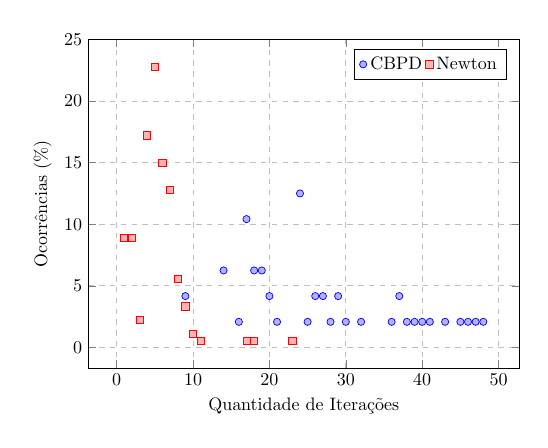
\begin{tikzpicture}[scale = 0.65]
  \begin{axis}[
    width=10cm,
    height=8cm,
    xlabel={Quantidade de Iterações},
    ylabel={Ocorrências (\%)},
    legend style={at={(0.5,-0.2)}, anchor=north, legend columns=-1},
    grid=major,
    grid style=dashed,
    legend pos=north east
  ]

    % First set of data
    \addplot[
      only marks,
      mark=*,
      color=blue,
      fill=blue!30,
    ] coordinates {
      (19, 6.25)
      (18, 6.25)
      (20, 4.17)
      (16, 2.08)
      (14, 6.25)
      (27, 4.17)
      (28, 2.08)
      (30, 2.08)
      (26, 4.17)
      (47, 2.08)
      (21, 2.08)
      (45, 2.08)
      (25, 2.08)
      (29, 4.17)
      (39, 2.08)
      (38, 2.08)
      (37, 4.17)
      (40, 2.08)
      (46, 2.08)
      (41, 2.08)
      (43, 2.08)
      (32, 2.08)
      (48, 2.08)
      (36, 2.08)
      (24, 12.50)
      (17, 10.42)
      (9, 4.17)
      };

    % Second set of data
    \addplot[
      only marks,
      mark=square*,
      color=red,
      fill=red!30,
    ] coordinates {
      (6, 15.00)
      (5, 22.78)
      (4, 17.22)
      (2, 8.89)
      (7, 12.78)
      (3, 2.22)
      (8, 5.56)
      (9, 3.33)
      (18, 0.56)
      (23, 0.56)
      (10, 1.11)
      (11, 0.56)
      (1, 8.89)
      (17, 0.56)
    };
    \legend{CBPD, Newton}

  \end{axis}
\end{tikzpicture}
\end{center}
